\chapter{Sviluppo del modulo nfproxy}

Come già esplicitato in prcedenza, il regex filtering è un modello di filtraggio che permette si ottime prestazioni (pochè processato, e costruito con linguaggi
e librerie veloci e low level), ma presentava delle grandi limitazioni in termini di flessibilità nell'analisi delle richieste e delle risposte, anche considerando che
la maggior parte dei servizi in ambito CTF girano su protocolli quali HTTP o a spesso unicamente su canali TCP, per esporre interfacce di programmi da terminale,
che spesso hanno parte dei loro contenuti compressi o rappresentati tramite encoding i quali contenuti non sono facilmente analizzabili tramite regex. \\

Al costo di prestazioni inferiori, con il vantaggio di poter scrivere i filtri in un linguaggio di semplice utilizzo e rapido per lo scripting quale
\texttt{Python}\footcite{\url{http://python.org/}}{python}, \texttt{nfproxy} è stato sviluppato proprio ai fin di superare i precedenti limiti lasciando una
estesa libertà nell'implementazione delle logiche di filtraggio del traffico,
mantenendo comunque un ottimo livello di prestazioni grazie ad alcune scelte architetturali intraprese e a diversi strumenti di sviluppo descritti in seguito.\\

\texttt{Nfproxy} non è propriamente di per se un proxy, ma un modulo che sfrutta l'utilizzo di
\texttt{nfqueue}\footcite{\url{https://netfilter.org/projects/libnetfilter_queue/}}{netfilter_queue} lasciando un grado di controllo sul traffico e una facilità di utilizzo
paragonabili a quella di un tradizionale proxy, dando in aggiunta accesso diretto ai pacchetti a livello di rete e inoltre non presenta le problematiche di
cambio di configurazione del servizio originale per applicare i filtri, poichè il traffico viene intercettato in
maniera totalmente invisibile, non richiedendo pertanto alcuna modifica sull'applicativo.\\
Si noti tuttavia come questa implementazione presenti alcune limitazioni riguardo la modifica, che però non rappresentano un scenario di utilizzo necessario
e strettamente utile per la difesa stessa del servizio. La parte che gestisce la queue come vedremo in seguito, è sviluppata tramite un utilizzo ibrido
di \texttt{C++} e \texttt{Python}, al fine di sfruttare alcune caratteristiche e librerie di \texttt{C++} per la gestione dei pacchetti, e permettere
l'utilizzo di python per il parsing ed il filtraggio dei pacchetti.
Il modulo supporta nativamente il parsing di HTTP/1.1\footcite{RFC2616, Hypertext Transfer Protocol -- HTTP/1.1}{rfc2616}, Websocket\footcite{RFC6455, The WebSocket Protocol}{rfc6455} e del normale flusso TCP\footcite{RFC9293, Transmission Control Protocol (TCP)}{rfc9293}.

\section{Requisiti}

Di seguito si elencano i requisiti principali, obiettivi dello sviluppo del seguente modulo:

\begin{itemize}
    \setlength{\itemsep}{5pt}
    \setlength{\parskip}{5pt}
    \item \texttt{Utilizzo del linguaggio python per la scrittura dei filtri}: il modulo deve offrire come strumenti di sviluppo dei filtri
    il linguaggio python, tramite l'ausilio di funzionalità offerte dal modulo stesso, ottimali, semplici per l'utilizzo per la scrittura dei filtri.
    \item \texttt{Supporto ai protocolli HTTP/1.1 e Websocket}: il modulo deve supportare nativamente il parsing dei pacchetti HTTP/1.1 e Websocket eseguendone il parsing
    e rendendo disponibili i dati già decodificati e decodificati quando è possibile, garantendone un accesso immediato. Deve supportare pertando i metodi di decompressione
    quali \texttt{gzip}\footcite{RFC1952, GZIP file format specification version 4.3}{rfc1952},
    \texttt{deflate}\footcite{RFC1951, DEFLATE Compressed Data Format Specification version 1.3}{rfc1951},
    \texttt{brotli}\footcite{RFC7932, Brotli Compressed Data Format}{rfc7932},
    \texttt{zstd}\footcite{RFC8478, Zstandard Compression and the application/zstd Media Type}{rfc8478}.
    Deve supportare anche l'estensione per websocket \texttt{permessage-deflate}\footcite{RFC7692, Compression Extensions for WebSocket}{rfc7692}.
    \item \texttt{Supporto al parsing dei pacchetti TCP}: il modulo deve supportare il parsing dei pacchetti TCP, permettendo l'accesso ai dati di livello di trasporto con payload già ordinati.
    \item \texttt{Accesso agli header ai livelli di rete e di trasporto}: il modulo deve permettere degli header IP e TCP accessibili e modificabili.
    \item \texttt{Supporto a IPv4 e IPv6}: il modulo deve supportare il parsing dei pacchetti IPv4\footcite{RFC791, Internet Protocol}{rfc791} e IPv6\footcite{RFC2460, Internet Protocol, Version 6 (IPv6) Specification}{rfc2460}.
    \item \texttt{Gestione autonoma dei buffer}: il modulo deve gestire autonomamente i buffer di memoria, evitando di sovraccaricare la memoria del sistema e di
    delegare la gestione di questi al programmatore, tuttavia lasciando la libertà di decisione sulle modalità di gestione, fornendo delle opzioni di configurazione opzionali.
    \item \texttt{Segnalazione degli errori}: il modulo deve segnalare in maniera chiara e precisa gli errori di parsing e di esecuzione dei filtri, facendo noto 
    al programmatore errori inaspettati rilevati e fornendo i log necessari per la risoluzione.
    \item \texttt{Supporto alla gestione dei filtri in maniera immediata}: deve essere possibile disabilitare totalmente o parzialmente i filtri in maniera immediata e
    senza downtime del servizio.
    \item \texttt{Supporto alla paralelizzazione}: il modulo deve supportare la paralelizzazione dei pacchetti, permettendo di sfruttare al meglio le risorse del sistema
    e garantendo un'ottima scalabilità del firewall.
    \item \texttt{Possibilitò di verifica del filtro tramite simulazione}: il modulo deve permettere di verificare il filtro in maniera simulata, permettendo di testare
    il quest'ultimo senza dover necessariamente applicarlo direttamente al traffico della macchina, permettendone il debugging e lo sviluppo in modo sicuro e rapido.
  \end{itemize}

\section{Architettura}

Il modulo nfproxy è avviato dal backend di firegex, che si occupa a sua volta di impostare le regole di \texttt{nftables}\footcite{\url{https://netfilter.org/projects/nftables/}}{nftables} tramite le sue API json,
avviare il modulo c++ dove viene gestita tutta la logica principale di multithreading, gestione dei pacchetti, assemblaggio dei payload
TCP e parsing del livello applicativo ed infine alla applicazione dei filtri python.\\
Di seguito un diagramma dell'architettura del modulo nfproxy, le varie componenti verranno analizzate nel dettaglio in seguito:

\begin{figure}[H]
    \centering
    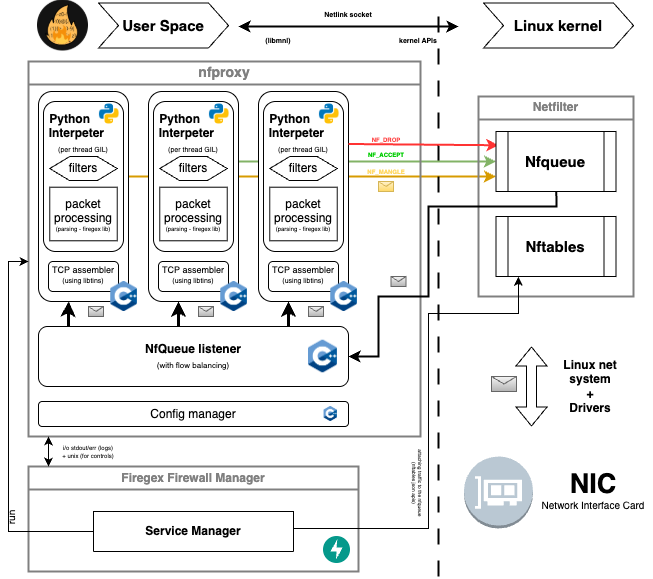
\includegraphics[width=0.9\textwidth]{images/chapter3/nfproxy.drawio.png}
    \caption{Architettura del modulo nfqueue}
    \label{fig:firegex_arch}
\end{figure}



\section{Elaborazione parallelizzata dei pacchetti}

Descrizione delle varie problematiche riguardo la parallelizzazione

\subsection{A Per-Interpreter GIL con python 3.12}

PEP 684

- https://peps.python.org/pep-0684/

\subsection{limiti sulla paralelizzazione di nfqueue}

- citazioni sul codice kernel per l'hash di ip

\subsection{Implementazione finale}

- citare parti di codice di nfproxy

\section{Parsing dei pacchetti L3}

Descrizione del parsing dei pacchetti L3 (libtins)

- https://libtins.github.io/

\section{Gestione dei pacchetti TCP}

Descrizione del problema della gestione del flusso TCP e soluzione adottata

\section{Modifica dei pacchetti}

Descrizione della modifica dei pacchetti e delle problematiche riscontrate

\subsection{Traduzione di ack e seq}

Descrizione della traduzione di ack e seq

\subsection{Modifica di segmenti non ordinati}

Descrizione del problema dei segmenti non ordinati con elenco dei problemi e proposta di soluzione.
Motivazione per l'incompletezza della soluzione.

- Riferimento agli sviluppi futuri

\section{Parsing dei pacchetti HTTP}

Descrizione del parsing dei pacchetti HTTP e delle problematiche riscontrate

Riferimento all'RFC

- \url{https://github.com/domysh/pyllhttp}

\subsection{Supporto agli algoritmi di compressione HTTP}

Riferimento all'RFC

- \url{https://github.com/domysh/brotli}

- \url{https://github.com/domysh/python-zstd}
    
\subsection{Supporto alle websocket}

Descrizione del supporto alle websocket

- \url{https://websockets.readthedocs.io/en/stable/}

\section{Sintassi e gestione dei filtri python}

Gestione dei dati, e sintassi adottata per la scrittura dei filtri

\subsection{Gestione dei buffer di memoria}

Descrizione della gestione sull' 'accumulo' dei buffer in memoria

\subsection{Gestione di encoding errati}

Descrizioni delle opzioni di gestione degli encoding errati

\section{Proxy di simulazione}

Descrizione del proxy di simulazione (comando fgex)
